
\documentclass[12pt]{article}
\usepackage{graphicx}
\usepackage{hyperref}
\usepackage{amsmath}


\begin{document}

\begin{center}
\textbf{ MAT 442: HMW5}\\
\textbf{\ ERICAGYEMANG (Spring 2019)}\\
\end{center}

\begin{enumerate} 
\item Example 3 on page 7, we check the stability of the 2-cycle for the \textbf{Ricker model}: For $a=9$ , $b=5$ and \[y_{k+1}=ay_ke^{-by_k},  \hspace{0.5cm}a>1.\]
Using the cobweb method we obtain

\begin{figure} [ht!]
 \centering
 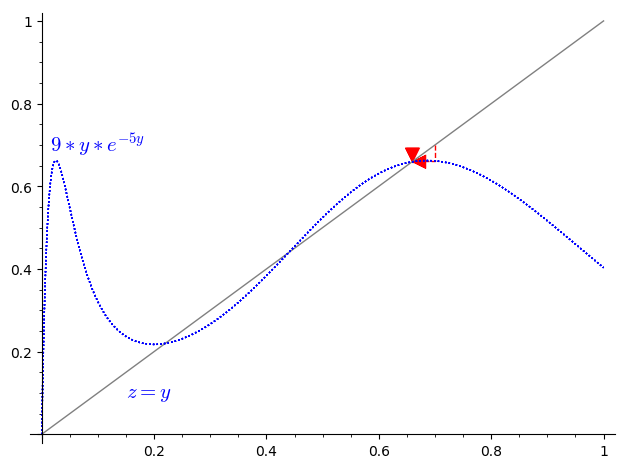
\includegraphics[height=3.5in]{/Users/ERICAGYEMANG/Desktop/Biomath/Figures/tmp_51.jpg} 
        \caption[Figure 2.4: r>1]{Cobweb diagram with r = 0.7}
 \label{fig::model}
\end{figure}
        
\begin{figure} [ht!]
 \centering
 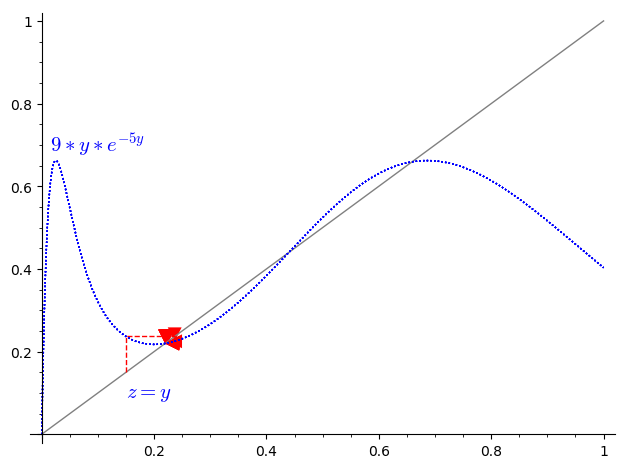
\includegraphics[height=3.5in]{/Users/ERICAGYEMANG/Desktop/Biomath/Figures/tmp_52.jpg} 
        \caption[Figure 2.4: r>1]{The cobweb diagram above is to show the stability of our 2-cycle. From our LN on periodic doubling and chaos we know that the orbit of 2-cycle point is also called a 2-cycle.Looking at the graph we see that there are four intersection, two of which must be the fixed points and the remaining two is a 2-cycle.The equilibrium points are \{$0$,$17/40$\} and we found that \{$1/5$,$13/20$\} is the 2-cycle.Looking at the graph, we clearly can see the cobweb attracting towards $11/50$.One interesting thing about how this attraction is that, it depends on the $r$.Let say if we chose our $r=0.7$ like in figure 1 above the cobweb will be attracting to $13/20$ which satisfies the fact that, if one point is attracting others will attract.}
 \label{fig::model}
\end{figure}

\cleardoublepage

\item We find all the equilibrium points and 2-cycles for DE\\
\[y_{k+1}=-\frac{1}{2}y^2_k-y_k+\frac{1}{2}.\]
To find equilibrium points, set
\begin{align*}
&f(y)=-\frac{1}{2}y^2-y+\frac{1}{2}\\
&\Rightarrow -\frac{1}{2}y^2-y+\frac{1}{2}=y\\
&\Rightarrow -\frac{1}{2}y^2-y+\frac{1}{2}-y=0\\
&\Rightarrow -2(-\frac{1}{2}y^2-2y+\frac{1}{2})=0\\
&\Rightarrow y^2+4y-1=0
\end{align*}
Using the quadratic formula we obtain
\begin{align*}
y&=\frac{-4 \pm \sqrt{4^2-4(1)(-1)}}{2(1)} \\
&=\frac{-4 \pm \sqrt{20}}{2}\\
&=\boxed{-2 \pm \sqrt{5}}.
\end{align*}
The derivative of
\[f(y)=-\frac{1}{2}y^2-y+\frac{1}{2}\]
is
\[\boxed{f'(y)=-y-1}.\]
Then
\[f'(y^1_\infty)=-(-2+\sqrt{5})-1=2-\sqrt{5}-1=1-\sqrt{5}\]
and 
\[f'(y^2_\infty)=-(-2-\sqrt{5})-1=2+\sqrt{5}-1=1+\sqrt{5}.\]
Now to check whether the fixed points its stable or unstable, we set
\[\left|f'(y^2_\infty )\right|=\left|1+\sqrt{5}\right|=\left|3.236\right|>1\]
Hence, our fixed points $y^1_\infty \mbox{,} y^2_\infty$ are unstable.To check the stability of 2-cycle, we have
\[\left| f'(-1)f'(1)\right|= \left|(1-1)(-2)\right|=\left|(0)(-2)\right|=\boxed{0<1}\]
Therefore the 2-cycle is LAS.

\cleardoublepage 



\item Finding the values of $a$, $b$ $\in$  $\rm I\!R$ for which \{$0,1$\} is an LAS 2-cycle for the function
\[f(y)=ay^3-by+1\]
we set
\begin{align*}
&f(y)=ay^3-by+1=y\\
&\Rightarrow ay^3-by+y+1=0\\
&\Rightarrow  ay^3-(b+1)y+1=0.
\end{align*}
Now substitute $0$ and $1$ into our function to obtain
\[f(0)=a(0)^3+b(0)+1=1\]
and
\[f(1)=a(1)^3+b(1)+1=a+b\Rightarrow a=b-1\]
so clearly there is some relation between $a$ and $b$.\\

We compute the derivative of $f$  
\[f'(y)=3ay^2-b\]
then
\[f'(0)=-b=-(a+1)=-a-1\hspace{0.3cm} (\mbox{because} \hspace{0.1cm}a+1=b)\]
and
\[f'(1)=3a-b=3a-a-1=2a-1.\]

Now we consider
\[\left|f'(0)f'(1)\right|=(-a-1)(2a-1)=-2a^2+a-2a+1=-2a^2-a+1.\]
and as always we set
\[-1<-2a^2-a+1<1\Leftrightarrow \boxed{ 0<2a^2+a<2}\]\\
Since we have LHS(case 1) and RHS(case 2) of the inequality, we consider 

\textbf{Case 1} : \boxed{0<2a^2+a} we know that coefficient of $a^2$ is greater zero which gives an open up parabola shape.
 
 \textbf{Case 2} : \boxed{2a^2+a<2} using the quadratic formula we derive 
  \[a\in\left(\frac{-1-\sqrt{17}}{4},\frac{-1+\sqrt{17}}{4}\right)\]
  
 Now we merge the solutions of both cases by union in order to know which interval $a$ and $b$ belongs to, so we obtain
\[a\in\left(-\frac{1}{2},\frac{-1-\sqrt{17}}{4}\right)\cup\left(0,\frac{-1+\sqrt{17}}{4}\right).\]

Because $a+1=b$,we also get
\[b\in\left(\frac{3-\sqrt{17}}{4},\frac{1}{2}\right)\cup\left(1,\frac{3+\sqrt{17}}{4}\right).\]

\cleardoublepage

\item Graphically deciding whether there are 3-cycles  for the discrete logistic model
\[y_{k+1}=3.828x(1-x).\]

a. Using the cobweb method, we get

\begin{figure} [ht!]
 \centering
 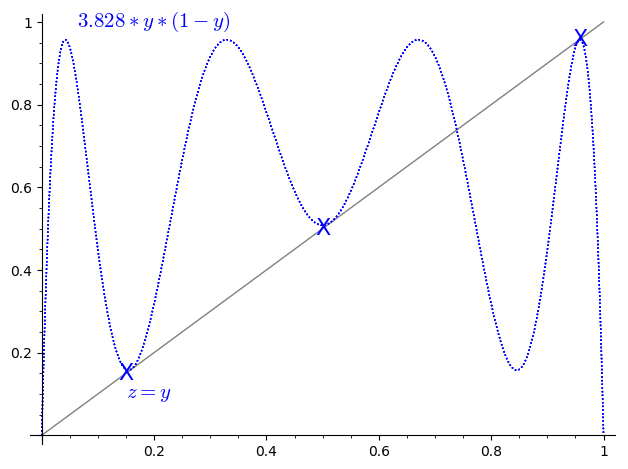
\includegraphics[height=4.5in]{/Users/ERICAGYEMANG/Desktop/Biomath/Figures/tmp_53.jpg} 
\caption[Figure 2.4: r>1]{The graph above shows the existence of 3-cycle.We can clearly see our curve intersecting with line $z=y$ at various points on the graph.I have marked the various points with X on the graph for easy indication.}
 \label{fig::model}
\end{figure}
\cleardoublepage

b. From the graph above we can see that our 3-cycles are \{0.2,0.5,1.0\} which is approximated numerical values for the 3-periodic points seen on the graph(which is marked in X).



\end{enumerate}

\cleardoublepage

\begin{thebibliography}{99}
\bibitem{r1}Dynamical Systems for Biological Modeling: An Introduction by Brauer and Kribs, CRC Press, 2016. ISBN 978-1-4200-6641-8


\end{thebibliography}

\end{document}